\chapter{روش پیشنهادی}
\clearpage

\section{روش مود مچینگ:}
سازه های موجدار با ناپیوستگی های طولی در بسیاری از کاربردها نقش دارند. تجزیه و تحلیل ناپیوستگی های راهنمای موج از اهمیت بالایی برخوردار است. یک رویکرد قدرتمند ، روش تطبیق حالت \lr{(MMT)} است که با استفاده از آن حالتهای موجی راهنما زمینه ها را توصیف می کنند و سپس شرایط مرزی که باید زمینه های مماس در سطح مقطع ساختار هدایتگر موج داشته باشند ، در رابط اعمال می شوند. بین بخشهای مختلف موجبر. در \lr{MMT} ، ساختار مورد بررسی به زیرسازی های ساده تری تقسیم می شود که حالت های آن (ویژه توابع ) مشخص است یا می توان آنها را تعیین کرد. میدان های الکتریکی و مغناطیسی ناشناخته با مجموع حالت های ویژه با ضرایب ناشناخته تقریبی می شوند. وقتی این عملکردها حالت عادی دارند ، از آنها به عنوان حالت های طبیعی یاد می شود. گسترش سری ، همه شرایط مرزی مشکل را برآورده می کند ، به جز مواردی که در رابط های بین مناطق فرعی مجاور وجود دارد. سپس ضرایب انبساط ناشناخته از شرایط مرزی در رابط ها تعیین می شود.
\begin{figure*}
    \centering
    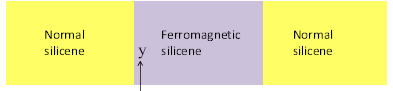
\includegraphics[width=\linewidth]{vallyschmatic.png}
    \caption{اتصال سیلیسین معمولی / فرومغناطیسی / معمولی}
    \label{fig:vallyschmatic}
\end{figure*}
ترابرد ، دره و اسپین را در یک اتصال سیلیسن طبیعی / فرومغناطیسی / طبیعی در \cite{yokoyamaControllableValleySpin2013} بررسی شده است. \gls{Yokoyama} نشان داده است که رسانایی بار ، دره و اسپین در این محل اتصال با طول سیلیسن فرو مغناطیسی نوسان می کند.

ماتریس انتقال و الگوریتم \gls{Lopez Sancho} برای محاسبه ترابرد
از آنجایی که در توضیح اثرات ابرشبکه بر روی خواص ترابرد ترکیبات دو بعدی از روش ماتریس انتقال استفاده خواهیم کرد در زیر به مرور نحوه کاربرد این مدل برای توصیف سیتمهای ساده تر مثل گرافین تک لایه تحت تأثیر پتانسیل پله ای دوره ای به نحوی که در شکل \ref{fig:vallyschmatic} مشخص گردید، می‌پردازیم.

قسمت بالایی شکل طیف انرژی شبه ذرات را در طول گرافین تک لایه نشان می‌دهد. از آنجایی که انرژی فرمی بین دو نوار گرافینی کنار هم متفاوت است، الگوی پتانسیل سیستم به شکل چاه های پتانسیل متوالی با استفاده از رابطه زیر قابل توصیف است

\begin{equation}
	V(x) = \begin{cases}
    V_0 &\quad l_{(2i-1)< |x| < l_{2i}\quad i=1,2,\dots}\\
    0 &\quad\text{\lr{Otherwise}}
\end{cases}
\end{equation}

این شکل پتانسیل مشابه همان شکلی است که در ابرشبکه های مبتنی بر نیمرسانا های معمولی اتفاق می‌افتد. تفاوت اساسی سیستم ما در این خواهد بود که رفتار حامل های بار به جای معادله شرودینگر از معادله دیراک تبعیت می‌کند که همیلتونی آن را می‌توان به شکل زیر نوشت

\begin{equation}
	\hat{H} = -i\hbar v_F\sigma \nabla + V(x)
    \label{eq:effectivehamiltonain}
\end{equation}
که در آن $v_f = 106 \; m/s$ سرعت فرمی و$\sigma(\sigma_x,\sigma_y)$ ماتریس های پائولی هستند. الکترونها و حفره‌ها در نیمرساناها معمولا توسط دو معادله شرودینگر جداگانه که با یکدیگر ارتباطی ندارند توصیف می‌شوند. اما در سیستم های دو بعدی نظیر این سیستم الکترون‌ها و حفره‌ها رفتار مرتبط با یکدیگر دارند و دارای خصوصیات کایرال می‌باشند. به این ترتیب که با یک تابع موج دو مؤلفه‌ای (توابع اسپینور) توصیف می‌شوند.

برای محاسبه ترابرد سیستمی که با همیلتونی رابطه \ref{eq:effectivehamiltonain} توصیف می‌شود، با در نظر گرفتن پاسخ کلی به صورت موج تختی که با زاویه معینی در جهت ابرشبکه حرکت می‌کند، مؤلفه‌های اسپینور دیراک بدست می‌آید. سپس با اعمال شرط پیوستگی تابع موج در مرز بین نوارهای مختلف ماتریس انتقال در صفحه دو ناحیه مجاور بدست می‌آید. از حاصلضرب ماتریس‌های انتقال ماتریس انتقال ابرشبکه به صورت زیر حاصل می‌شود:
\begin{equation}
    \begin{split}
    S(z) = S(z=l_{2}) = S(z=l_{3}) &= \dots S(z=l_{i})       \dots S(z=l_{n-1})\\
    S(z=l_{i}) &= 
        \begin{bmatrix} 
            t_{11} & t_{12} \\
            t_{21} & t_{22}
        \end{bmatrix}
    \end{split}
\end{equation}

به این ترتیب احتمال عبور موج به صورت تابعی از زاویه برخورد بدست می‌آید که برای این سیستم رابطه زیر بدست می‌آید:
\begin{equation}
    T(\phi) = \frac{e^{-2ik_x\prime D-q(D+L)(1+e^{2i\theta})^2(1+e^{2i\phi})^2}}{A_1^2 + B_1^2}
\end{equation}
پس از  بدست آمدن ضرایب عبور می‌توان با استفاده از رابطه \gls{Buttiker} رسانش سیستم را بدست آورد:
\begin{equation}
    G = G_0 \int_{-\pi/2}^{\pi/2} T(E,\sqrt{2E} sin\phi)cos\phi d\phi
\end{equation}
که در آن$G_0 = e^2m v_F w/\hbar^2$خواهد بود.

% \section{روش تابع گرین غیرتعادلی:}
% روش \gls{Lopez Sancho} برای محاسبه ترابرد در سیستمهایی که در یک بعد شرط مرزی بلاخ را رعایت می‌کنند دارای همگرایی بالایی است و توان محاسباتی کمی نیاز دارد. برای توضیح روش فرض می‌کنیم یک نانونوار گرافینی در یک بعد دارای ساختار تناوبی می‌باشد. ابتدا باید به کمک هامیلتونی \lr{TB} ماتریس برهمکنش یک سوپرسل با خودش $H_{0,0}$ را محاسبه و همچنین برهمکنش یک سوپرسل با سلول مجاورش$H_{0,1}$ را محاسبه کنیم.


% حال به کمک ماتریس هاي فوق و روش لوپز خود انرژي الکترودهاي طرفین را محاسبه می‌کنیم. براي این کار ابتدا توابع گرین سطحی الکترودها را محاسبه می‌کنیم.
% \begin{equation}
%     \begin{split}
%         g_{0,0}^L = \left[ E^{+}I - H_{0,0} -H^{\dagger}_{-1,0} \right]^{-1}\\
%         g_{M+1,M+1}^R = \left[ E^{+}I - H_{0,0} -H^{\dagger}_{-1,0} \right]^{-1}
%     \end{split}
% \end{equation}
% در روابط فوق $E^{+} = E + i\eta$  می‌باشدکه $\eta$ مقدار کوچکی است که برای فرار از تکینگی به کار می‌بریم. برای استفاده از روابط فوق نیاز داریم ماتریس های انتقال را محاسبه کنیم. برای این کار از یک روش تکرار استفاده می‌شود.
% \begin{equation}
%     \begin{split}
%         \Lambda = t_0 + \hat{t_0} t_1 + \hat{t_0}\hat{t_1}t_2 + \dots \hat{t_0}\hat{t_1}\hat{t_2}\dots t_n\\
%         \hat{\Lambda} = \hat{t_0} + t_0 \hat{t_1} + \hat{t_0}\hat{t_1}t_2 + \dots t_0 t_1 t_2\dots \hat{t_n}
%     \end{split}
% \end{equation}
% که در آن $t_i$ و $\hat{t_i}$  به نحو زیر تعریف می‌شوند:
% \begin{equation}
%     \begin{split}
%         t_i = \left(I-t_{i-1}\hat{t}_{i-1}-\hat{t}_{i-1}t_{i-1}\right)^{-1} t_{i-1}^2\\
%         \hat{t_i} = \left(I-t_{i-1}\hat{t}_{i-1}-\hat{t}_{i-1}t_{i-1}\right)^{-1} \hat{t}_{i-1}^2
%     \end{split}
% \end{equation}
% و به ازای مقدار $i = 0$ داریم:
% \begin{equation}
%     \begin{split}
%         t_0 = \left(E^{+}I-H_{0,0}\right)^{-1} H^{\dagger}_{-1,0}\\
%         t_0 = \left(E^{+}I-H_{0,0}\right)^{-1} H_{-1,0}
%     \end{split}
% \end{equation}
% با در نظر گرفتن سوپرسل نمونه به عنوان قسمتی از لید چپ به صورت لایه به لایه ( از $l = M$ تا $l = 2$) می‌توانیم تابع گرین سطحی را بدست آوریم:
% \begin{equation}
%     g_{l,l}^R = \left[E^+ I- H_{l,l} - H_{l,l}g_{l+1,l+1}^RH^{\dagger}_{l,l+1} \right]^{-1}
% \end{equation}
% پس از آن تابع گرین کل از رابطه زیر قابل محاسبه خواهد بود:
% \begin{equation}
%     G_{11} = \left[E^+I- H_{1,1}- \Sigma^L-\Sigma^R\right]
% \end{equation}
% که در آن: 
% \begin{equation}
%     \begin{split}
%         \Sigma^L = H^{\dagger}_{0,1} g^{L}_{0,0}H_{0,1}\\
%         \Sigma^R = H_{1,2} g^{R}_{2,2}H^{\dagger}_{1,2}
%     \end{split}
% \end{equation}
% خود انرژیهای مربوط به برهمکنش با لیدهای چپ و راست هستند. از تابع گرین می‌توان چگالی حالتهای جایگزیده \lr{(LDOS)} را نیز بدست آورد: 
% \begin{equation}
%     n_j = - \frac{1}{\pi} Im[G_{(j,j)}]
% \end{equation}
% که اندیس $j,j $به سایت مورد نظر اشاره می‌کند. در نهایت با استفاده از فرمول لانداور می‌تواند رسانش را بدست آورد:
% \begin{equation}
%     G_{(E)} = \frac{2e^2}{h} T_{(E)}
% \end{equation}
% که در آن از روابط زیر برای محاسبه احتمال عبور استفاده شده است: 
% \begin{equation}
%     \begin{split}
%         T_{(E)} = Tr[\Gamma^{L}G_{11}\Gamma^{R}G^{\dagger}_{1,1}]\\
%         \Gamma^{L,R} = i [\Sigma^{L,R}- (\Sigma^{L,R})^{\dagger}]
%     \end{split}
% \end{equation}
% به این ترتیب هزینه محاسباتی این سیستم  $2N x 2N$ به طور خطی با $N$ تغییر می‌کند. این روش را به راحتی می‌توان با تنظیم پارامترهای هاپینگ و آنسایت به ابر شبکه ها تعمیم داد به طوری که سوپر سل حاوی یک دوره تناوب ابر شبکه باشد.
\section{روش بازگشتی:}
\subsection{معادله دایسون:}

روش تابع گرین بازگشتی رویکردی برای محاسبه توابع گرین سیستم‌های چند جزئی است، در صورتی که توابع گرین زیرسیستم‌های ایزوله شده و ماتریس‌های جفت شدگی بین زیرسیستم‌ها شناخته شده باشند. با شروع از یک انتهای سیستم (معمولاً یکی از الکترودها)، زیرسیستم‌ها یکی یکی اضافه می‌شوند، در نهایت می‌توان تابع گرین کل سیستم را پیدا کرد. این یک روش راحت برای محاسبه مولفه‌های تابع گرین مربوطه برای سیستم‌های پیچیده بزرگ است که می‌توان آنها را به بخش‌های متصل زیادی تقسیم کرد. از دیدگاه محاسباتی، روش بازگشتی می‌تواند بسیار سریع‌تر از حل مستقیم معادلات برای سیستم‌های بزرگ باشد.
این روش بر اساس معادله دایسون برای تابع گرین کامل $G$، تابع گرین برای یک سیستم جدا شده $G_0$ و ماتریس جفت شدگی $V$ است:
\begin{equation}
    \mathbf{G}={{\mathbf{G}}_{0}}+{{\mathbf{G}}_{0}}\mathbf{VG}.
\end{equation}
$G_F$ کامل با هامیلتونی کامل $H = H_0 + V$ تعریف می شود: $(E - H) G = I$، $G_F$ قسمت های خاص سیستم به صورت $(E - H_0) G_0 = I$ تعریف می‌شود. با مقایسه این دو معادله، بدست آوردن آن آسان است$\left(E-H_0-V\right)G=I\rightarrow\left(E-H_0\right)G-VG=I\rightarrow\left(E-H_0\right)G_0G-G_0VG=G_0\rightarrow G-G_0VG=G_0$
مزیت معادله دایسون این است که اگر یک سیستم خارجی اضافی را به سیستم مورد نظر متصل کنیم، کافی است تابع گرین این سیستم خارجی (مستقل از نحوه محاسبه آن) و ماتریس جفت شدن را بدانیم. توجه داشته باشید که این رویه فقط برای سیستم‌های غیر برهمکنشی یا به‌عنوان اختلال \lr{V} برای سیستم‌های برهمکنشی کار می‌کند، در غیر این صورت \lr{V} باید با یک خود انرژی عمومی‌تر جایگزین شود. با این حال، روش بازگشتی را می توان برای سیستم های برهمکنشی در ترکیب با روش تکراری اعمال کرد.

در نظر بگیرید که اگر دو سیستم را با توابع گرین $G_0 A$ و $G_0B$ جفت کنیم (شکل 3-3) این معادله چگونه کار می کند، توجه داشته باشید که برای زیرسیستم های $A$ و $B$ نیازی به همیلتونی صریح نداریم، آنها می توانند به هر تعداد دلخواه سیستم های دیگر و نیز الکترودها از طریق خود انرژی مربوطه متصل شوند. توابع $G0A$ و $G0B$ در زیرفضاهای $A$ و $B$ به ترتیب با تعداد حالت های $NA$ و $NB$ تعریف می شوند، ماتریس های کامل $G$ $G_0$، $V$ دارای ابعاد $(NA + NB) \times (NA + NB)$ هستند و ما معادله (3.1)به صورت زیر می نویسیم:
\begin{equation}
    \left( \begin{matrix}
           {{G}_{A}} & {{G}_{AB}}  \\
           {{G}_{BA}} & {{G}_{B}}  \\
        \end{matrix} \right)=\left( \begin{matrix}
           G_{A}^{0} & 0  \\
           0 & G_{B}^{0}  \\
        \end{matrix} \right)+\left( \begin{matrix}
           G_{A}^{0} & 0  \\
           0 & G_{B}^{0}  \\
        \end{matrix} \right)\left( \begin{matrix}
           0 & {{V}_{AB}}  \\
           {{V}_{AB}} & 0  \\
        \end{matrix} \right)\left( \begin{matrix}
           {{G}_{A}} & {{G}_{AB}}  \\
           {{G}_{BA}} & {{G}_{B}}  \\
        \end{matrix} \right),
\end{equation}

که در آن $V_{AB}$ ماتریس جفت شدگی بین زیرسیستم‌ها با ابعاد $N_A\times N_B$ است. ما علاقه مند به محاسبه تابع \lr{GA} هستیم که زیرسیستم $A$ را توصیف می کند و $G_{BA}$ جفت شدگی بین زیرسیستم های $A$ و $B$ را توصیف می کند. پس از محاسبات ساده به دست می آوریم
\begin{equation}
    \begin{split}
          & {{G}_{A}}=G_{A}^{0}+G_{A}^{0}{{V}_{AB}}{{G}_{BA}}\qquad {{G}_{AB}}=G_{A}^{0}{{V}_{AB}}{{G}_{B}} \\ 
         & {{G}_{BA}}=G_{B}^{0}{{V}_{BA}}{{G}_{A}}\qquad \qquad {{G}_{B}}=G_{B}^{0}+G_{B}^{0}{{V}_{BA}}{{G}_{AB}} \\ 
         & {{G}_{A}}=G_{A}^{0}+G_{A}^{0}{{V}_{AB}}{{G}_{BA}}\qquad {{G}_{AB}}=G_{A}^{0}{{V}_{AB}}{{G}_{B}} \\ 
        & {{G}_{BA}}=G_{B}^{0}{{V}_{BA}}{{G}_{A}}\qquad \qquad {{G}_{B}}=G_{B}^{0}+G_{B}^{0}{{V}_{BA}}{{G}_{AB}} \\ 
    \end{split}
\end{equation}
ما محاسبه خود انرژی را به شیوه ای کلی تر از (3.120) بازتولید می کنیم 
\begin{equation}
    {{\Sigma }_{AB}}={{V}_{AB}}G_{B}^{0}{{V}_{BA}},
\end{equation}

توسط سیستم $B$ وارد سیستم $A$ شده است.
به عنوان یک مثال دیگر ثابت می کنیم که خود انرژی چند الکترودی (3.122) مجموع خود انرژی های الکترودهای خاص است. فرض کنید یک الکترود دیگر با تابع گرین (الکترود ایزوله) $G_s$ از طریق ماتریس جفت شدگی $V_{sC}$ اضافه می کنیم. تابع گرین سیستم قبلی $G(0)C= [E−HC−Σ(0)]^{-1}$ است که $\Sigma(\theta)$خود انرژی تمام الکترودهایی است که قبلا جفت شده اند. با استفاده از معادله (3.3) بدست می آوریم
\begin{equation}
    \left( {{\left( G_{C}^{0} \right)}^{-1}}-{{V}_{Cs}}{{G}_{s}}{{V}_{sC}} \right){{G}_{C}}=\left( E-{{H}_{C}}-{{\Sigma }^{(0)}}-{{\Sigma }_{Cs}} \right){{G}_{C}}=I,
\end{equation}

به طوری که خود انرژی جدید $\Sigma ={{\Sigma }^{(0)}}+{{\Sigma }_{C\ s}}$ باشد. 
روش بازگشتی برای سیستم های $1$ بعدی:
محاسبه مستقیم تابع گرین ریتاردد با استفاده از وارونگی ماتریس (3.118) ممکن است از نظر محاسباتی برای سیستم های بزرگ غیرقابل حل باشد. در مورد بسیار مهم سیستم‌های "طولانی" با نسبت طول به عرض بالا و جفت شدن کوتاه برد بین اوربیتال‌های پایه (نمونه‌های مهم نانولوله‌های کربنی و نانوروبان‌ها) سیستم مرکزی را می‌توان به بسیاری از بخش‌ها (برش‌ها) تقسیم کرد که فقط همسایه‌ها بین برش‌ها جفت می‌شوند (شکل 3.4)، یعنی $H_{i,i+1}$ جفت شدن برش $i$ و $(i + 1)$ است. همیلتونی شکل سه قطری دارد:
\begin{equation}
    H=\left( \begin{matrix}
           {{H}_{11}} & {{H}_{12}} & 0 & \ldots  & 0  \\
           {{H}_{21}} & {{H}_{22}} & {{H}_{23}} & \ldots  & 0  \\
           0 & {{H}_{32}} & {{H}_{33}} & \ldots  & 0  \\
           \vdots  & \vdots  & \vdots  & \ddots  & {{H}_{N,N-1}}  \\
           0 & \ldots  & 0 & {{H}_{N-1\ N}} & {{H}_{NN}}  \\
        \end{matrix} \right),
\end{equation}

علاوه بر این، در اینجا فرض می‌کنیم که برش‌های $1$ و $N$ به ترتیب توسط انرژی‌های $\Sigma_L$ و $\Sigma_R$ به الکترودهای چپ و راست جفت می‌شوند.
تابع گرین $G$ را می توان به عنوان یک ماتریس در "فضای برش" با عناصر ماتریس بر اساس برش های مربوطه نشان داد:
\begin{equation}
    G=\left( \begin{matrix}
           {{G}_{11}} & {{G}_{12}} & {{G}_{13}} & \ldots  & {{G}_{1N}}  \\
           {{G}_{21}} & {{G}_{22}} & {{G}_{23}} & \ldots  & {{G}_{2N}}  \\
           {{G}_{31}} & {{G}_{32}} & {{G}_{33}} & \ldots  & {{G}_{3N}}  \\
           \vdots  & \vdots  & \vdots  & \ddots  & \vdots   \\
           {{G}_{N1}} & {{G}_{N2}} & {{G}_{N3}} & \ldots  & {{G}_{NN}}  \\
        \end{matrix} \right),
\end{equation}
تابع گرین کامل را می توان از معادله زیر پیدا کرد
\begin{equation}
    \left( E-H-\Sigma  \right)G=I,
\end{equation}
که در آن خود انرژی الکترود فقط دو مولفه در فضای برش دارد: $\Sigma_{11} = \Sigma_{L}$ و $\Sigma_{NN} = \Sigma_{R}$.
معمولاً محاسبه همه عناصر مورد نیاز نیست. در واقع، جایگزین کردن (3.142) در عبارات برای تابع رسانندگی (3.133) و چگالی محلی حالات (3.104) و در نظر گرفتن این که فقط اولین و آخرین برش‌ها به الکترودها جفت می شوند ($\Gamma_{L}$ فقط یک عنصر غیر صفر دارد ${{\Gamma }_{L,11}}=-2\operatorname{Im}\ {{\Sigma }_{L}}$ و ${{\Gamma }_{R,NN}}=-2\operatorname{Im}\ {{\Sigma }_{R}}$، پیدا می کنیم 
\begin{equation}
    \begin{split}
        T(E)=\underbrace{\left( \begin{matrix}
        -2\operatorname{Im}{{\Sigma }_{L}} & 0 & 0 & \ldots  & 0  \\
        0 & 0 & 0 & \ldots  & 0  \\
        0 & 0 & 0 & \ldots  & 0  \\
        \vdots  & \vdots  & \vdots  & \ddots  & \vdots   \\
        0 & 0 & 0 & \ldots  & 0  \\
        \end{matrix} \right)}_{{{\Gamma }_{L}}}\times \underbrace{\left( \begin{matrix}
        {{G}_{11}} & {{G}_{12}} & {{G}_{13}} & \ldots  & {{G}_{1N}}  \\
        {{G}_{21}} & {{G}_{22}} & {{G}_{23}} & \ldots  & {{G}_{2N}}  \\
        {{G}_{31}} & {{G}_{32}} & {{G}_{33}} & \ldots  & {{G}_{3N}}  \\
        \vdots  & \vdots  & \vdots  & \ddots  & \vdots   \\
        {{G}_{N1}} & {{G}_{2N}} & {{G}_{3N}} & \ldots  & {{G}_{NN}}  \\
        \end{matrix} \right)}_{{{G}^{R}}}\times  \\ 
        \underbrace{\left( \begin{matrix}
        {{G}_{11}} & {{G}_{21}} & {{G}_{31}} & \ldots  & {{G}_{N1}}  \\
        {{G}_{12}} & {{G}_{22}} & {{G}_{32}} & \ldots  & {{G}_{N3}}  \\
        {{G}_{13}} & {{G}_{23}} & {{G}_{33}} & \ldots  & {{G}_{N3}}  \\
        \vdots  & \vdots  & \vdots  & \ddots  & \vdots   \\
        {{G}_{1N}} & {{G}_{2N}} & {{G}_{3N}} & \ldots  & {{G}_{NN}}  \\
        \end{matrix} \right)}_{{{G}^{A}}}\times \underbrace{\left( \begin{matrix}
        0 & 0 & 0 & \ldots  & 0  \\
        0 & 0 & 0 & \ldots  & 0  \\
        0 & 0 & 0 & \ldots  & 0  \\
        \vdots  & \vdots  & \vdots  & \ddots  & \vdots   \\
        0 & 0 & 0 & \ldots  & -2\operatorname{Im}{{\Sigma }_{R}}  \\
        \end{matrix} \right)}_{{{\Gamma }_{R}}} \\
        \left( \begin{matrix}
        0 & 0 & 0 & \ldots  & (-2\operatorname{Im}{{\Sigma }_{L}})\ {{G}_{1N}}(-2\operatorname{Im}{{\Sigma }_{R}})\ {{G}_{N1}}  \\
        0 & 0 & 0 & \ldots  & 0  \\
        0 & 0 & 0 & \ldots  & 0  \\
        \vdots  & \vdots  & \vdots  & \ddots  & \vdots   \\
        0 & 0 & 0 & \ldots  & 0  \\
        \end{matrix} \right)
        T(E)=Tr\left({{\Gamma }_{L}}{{G}_{1N}}{{\Gamma }_{R}}G_{1N}^{\dagger} \right),
    \end{split}
\end{equation}
\begin{equation}
    \rho (E)=\sum\limits_{i=1}^{N}{{{\rho }_{i}}(E)}=-\frac{1}{\pi }\sum\limits_{i=1}^{N}{\operatorname{Im}(Tr\ {{G}_{ii}})}.
\end{equation}
همانطور که می بینید، برای محاسبه انتقال و جریان فقط $G_{1N}$ مورد نیاز است، برای محاسبه $DOS$ نیز تمام $G_{ii}$. 
توابع گرین را می‌توان با شروع از هر انتهایی محاسبه کرد، ابتدا جهت بازگشتی را از چپ به راست در نظر می گیریم (بازگشتی رو به جلو). در مرحله اول تابع گرین $G_{11}\rightarrow(1)$ است 
\begin{equation}
    G_{11}^{\to (1)}={{\left[ E-{{H}_{11}}-{{\Sigma }_{L}} \right]}^{-1}},
\end{equation}
این تابع $G_{11}$ تابعی که در (3.7) هست، نیست، بلکه فقط تابع اولین برش متصل به الکترود سمت چپ است (شکل 3.5). این روش را N بار برای توابع $G_{ii}\rightarrow(i)$ و $G_{1i}\rightarrow(i)$، برای $2<i<N$ تکرار می کنیم: 
\begin{equation}
    G_{ii}^{\to (i)}={{\left[ E-{{H}_{ii}}-{{\Sigma }_{R}}{{\delta }_{iN}}-{{H}_{i,i-1}}G_{i-1,i-1}^{\to (i-1)}\ {{H}_{i-1,i}} \right]}^{-1}}
\end{equation}
\begin{equation}
    G_{1i}^{\to (i)}=G_{1,i-1}^{\to (i-1)}\ {{H}_{i-1,i}}\ G_{ii}^{\to (i)}.
\end{equation}

معادله (3.12) از (3.3) به دست می‌آید.
\begin{equation}
‌   \begin{split}
          & \left[ \begin{matrix}
           G_{11}^{\to (1)} & G_{12}^{\to (1)}  \\
           G_{21}^{\to (1)} & G_{22}^{\to (2)}  \\
        \end{matrix} \right]=\left[ \begin{matrix}
           G_{11}^{\to (0)} & 0  \\
           0 & G_{22}^{\to (0)}  \\
        \end{matrix} \right]+\left[ \begin{matrix}
           G_{11}^{\to (0)} & 0  \\
           0 & G_{22}^{\to (0)}  \\
        \end{matrix} \right]\left[ \begin{matrix}
           0 & {{H}_{12}}  \\
           {{H}_{21}} & 0  \\
        \end{matrix} \right]\left[ \begin{matrix}
           G_{11}^{\to (1)} & G_{12}^{\to (1)}  \\
           G_{21}^{\to (1)} & G_{22}^{\to (2)}  \\
        \end{matrix} \right] \\ 
         & \left[ \begin{matrix}
           G_{11}^{\to (1)} & G_{12}^{\to (1)}  \\
           G_{21}^{\to (1)} & G_{22}^{\to (2)}  \\
        \end{matrix} \right]=\left[ \begin{matrix}
           G_{11}^{\to (0)} & 0  \\
           0 & G_{22}^{\to (0)}  \\
        \end{matrix} \right]+\left[ \begin{matrix}
           G_{11}^{\to (0)}{{H}_{12}}G_{21}^{\to (1)} & G_{11}^{\to (0)}{{H}_{12}}G_{22}^{\to (2)}  \\
           G_{22}^{\to (0)}{{H}_{21}}G_{11}^{\to (1)} & G_{22}^{\to (0)}{{H}_{21}}G_{12}^{\to (1)}  \\
        \end{matrix} \right] \\ 
        & G_{22}^{\to (2)}=G_{22}^{\to (0)}+G_{22}^{\to (0)}{{H}_{21}}G_{12}^{\to (1)} \\ 
        & G_{12}^{\to (1)}=G_{11}^{\to (0)}{{H}_{12}}G_{22}^{\to (2)}\left.\right\}\Rightarrow G_{22}^{\to (2)}=G_{22}^{\to (0)}+G_{22}^{\to (0)}{{H}_{21}}G_{11}^{\to (0)}{{H}_{12}}G_{22}^{\to (2)}\\
        &\left[ 1-G_{22}^{\to (0)}{{H}_{21}}G_{11}^{\to (0)}{{H}_{12}} \right]G_{22}^{\to (2)}=G_{22}^{\to (0)}\Rightarrow \left[ {{\left( G_{22}^{\to (0)} \right)}^{-1}}-{{H}_{21}}G_{11}^{\to (0)}{{H}_{12}} \right]G_{22}^{\to (2)}=I \\
        & G_{22}^{\to (2)}={{\left[ {{\left( G_{22}^{\to (0)} \right)}^{-1}}-{{H}_{21}}G_{11}^{\to (0)}{{H}_{12}} \right]}^{-1}}\Rightarrow G_{22}^{\to (2)}={{\left[ E-{{H}_{22}}-{{H}_{21}}G_{11}^{\to (0)}{{H}_{12}} \right]}^{-1}} 
    \end{split}
\end{equation}
برای به دست آوردن معادله (3.13) ما معادله دایسون (3.1) را که قبل از اتصال تکه $i$ام $G_0$ گرفته شده است در نظر می‌گیریم (فقط عناصر محاسبه شده با روش فوروارد را نشان می دهیم):
\begin{equation}
    {{G}_{0}}=\left( \begin{matrix}
        G_{11}^{\to (1)} & G_{12}^{\to (2)} & \ldots  & G_{1,i-1}^{\to (i-1)} & 0  \\
        {} & G_{22}^{\to (2)} & {} & {} & 0  \\
        {} & {} & \ddots  & {} & {}  \\
        {} & {} & {} & G_{i-1,i-1}^{\to (i-1)} & \vdots   \\
        0 & 0 & \ldots  & 0 & G_{ii}^{\to (0)}  \\
    \end{matrix} \right)
\end{equation}
و ماتریس جفت‌شدگی $V$ فقط دارای عناصر $V_{i-1,i} = H_{i-1,i}$ و $V_{i,i-1} = H_{i,i-1}$ است. از سطر و ستون  $i$-ام (3.1) بلافاصله معادله (3.13) به دست می‌آید.
\begin{equation}
    \left( \begin{matrix}
        G_{11}^{\to (1)} & G_{12}^{\to (2)} & \ldots  & G_{1i-1}^{\to (i-1)} & 0  \\
        {} & G_{22}^{\to (2)} & {} & {} & 0  \\
        {} & {} & \ddots  & {} & {}  \\
        {} & {} & {} & G_{i-1,i-1}^{\to (i-1)} & \vdots   \\
        0 & 0 & \ldots  & 0 & G_{ii}^{(0)}  \\
        \end{matrix} \right)\times \left( \begin{matrix}
        0 & 0 & 0 & \ldots  & 0 & 0  \\
        0 & 0 & 0 & \ldots  & 0 & 0  \\
        \vdots  & \vdots  & \vdots  & \ddots  & 0 & 0  \\
        0 & 0 & 0 & 0 & {{H}_{i-1,1}} & 0  \\
        0 & 0 & 0 & {{H}_{i,i+1}} & 0 & 0  \\
        \vdots  & \vdots  & \vdots  & \vdots  & \ddots  & \vdots   \\
    \end{matrix} \right)
\end{equation}
در هر مرحله $i$-امین تابع گرین برش $G_{ii}\rightarrow(i)$ و انتشار دهنده بین اولین و برش $i$-امین $G_{1i}\rightarrow{i}$ برای سیستم متصل به برش $i$-امین به الکترود سمت چپ را بدست می‌آوریم. در مرحله آخر، $G_{1N}\rightarrow(N)$ را بدست می‌آوریم، که تابع درست $G_{1N}$ است و برای محاسبه تابع انتقال کافی است، همانطور که از (3.9) مشاهده می‌شود.
تلاش محاسباتی اضافی برای محاسبه چگالی حالات (3.10) مورد نیاز است، زیرا فرد به تمام عناصر قطری $G_{ii}$ نیاز دارد، و در طی روند بازگشتی از چپ به راست، ما فقط توابع میانی $G_{ii}\rightarrow(i)$ را برای سیستم های جزئی بدست آوردیم. برای بدست آوردن سایر توابع گرین برش، روند بازگشتی به عقب را برای $N ≥ i ≥ 1$ اعمال می‌کنیم:
\begin{equation}
    G_{NN}^{\leftarrow (N)}={{\left[ E-{{H}_{N\ N}}-{{\Sigma }_{R}} \right]}^{-1}},
\end{equation}
% 	\[\]	(3.15)
\begin{equation}
    G_{i\ i}^{\leftarrow (i)}={{\left[ E-{{H}_{i\ i}}-{{\Sigma }_{L}}{{\delta }_{i1}}-{{H}_{i,i+1}}G_{i+1,i+1}^{\leftarrow (i+1)}{{H}_{i+1,i}} \right]}^{-1}},
\end{equation}
در پایان این روش، ما پاسخ درست را برای G11 دریافت می‌کنیم، و همچنانکه درروند بازگشتی به جلو که GNN به دست آوردیم، همه $G_{ii}$ های دیگر برای  $1≤ i ≤ N$ به صورت زیر محاسبه می شوند:
\begin{equation}
    \left[ \begin{matrix}
           {{G}_{11}} & {{G}_{12}}  \\
           {{G}_{21}} & {{G}_{22}}  \\
        \end{matrix} \right]=\left[ \begin{matrix}
           G_{11}^{\leftarrow (1)} & 0  \\
           0 & G_{22}^{\to (2)}  \\
        \end{matrix} \right]+\left[ \begin{matrix}
           G_{11}^{\leftarrow (1)} & 0  \\
           0 & G_{22}^{\to (2)}  \\
        \end{matrix} \right]\left[ \begin{matrix}
           0 & {{H}_{12}}  \\
           {{H}_{21}} & 0  \\
        \end{matrix} \right]\left[ \begin{matrix}
           {{G}_{11}} & {{G}_{12}}  \\
           {{G}_{21}} & {{G}_{22}}  \\
        \end{matrix} \right]
        G_{i\ i}^{{}}={{\left[ E-{{H}_{i\ i}}-{{H}_{i,i-1}}G_{i-1,i-1}^{\to (i-1)}{{H}_{i-1,i}}-{{H}_{i,i+1}}G_{i+1,i+1}^{\leftarrow (i+1)}{{H}_{i+1,i}} \right]}^{-1}}.
\end{equation}
این فقط معادله دایسون برای برش $i$ با خود انرژی های چپ و راست است. در واقع اولین قسمت در این عبارت قبلاً $[G_{ii}\rightarrow(i)]^{-1}$ محاسبه شده است. به طوری که ما می توانیم این عبارت را بازنویسی کنیم
\begin{equation}
    G_{i\ i}^{{}}={{\left[ I-G_{i,i}^{\to (i)}{{H}_{i,i+1}}G_{i+1,i+1}^{\leftarrow (i+1)}{{H}_{i+1,i}} \right]}^{-1}}G_{ii}^{\to (i)},
\end{equation}
برای سیستم های طولانی با برهمکنش کوتاه برد، زمان مورد نیاز برای مقیاس‌های محاسبه به عنوان $M3N$، که در آن $M\times M$ ابعاد معمولی یک ماتریس برش هستند (زمان معمولی وارونگی ماتریس $M3$ است). اگر کسی از وارونگی برای کل سیستم استفاده کند، آن را به صورت $(MN)3$ مقیاس می‌کند که برای $N$ بزرگ بسیار بزرگتر است.

\subsection{سیستم های با چند اتصال:}
در مورد سیستم‌های دوبعدی و سه‌بعدی چند اتصالی، اگر سیستم به برش‌هایی با چندین زیرسیستم در هر برش تقسیم شود، روش بازگشتی به شکلی که در بالا توضیح داده شد، می‌تواند اعمال شود. به طور متناوب، معادله دایسون را می توان برای سیستم‌های چند اتصالی با توابع گرین زیرسیستم های جدا شده در $G_0$ و تمام اتصالات بین زیرسیستم‌ها در $V$ اعمال کرد.
به عنوان مثال سه زیرسیستم بین دو الکترود را در نظر بگیرید (شکل 3.6). برش اول شامل زیرسیستم‌های $A$ و $B$ دومی شامل زیرسیستم $C$ است. انرژی $\Sigma_{L}$ باید برای سیستم $A + B$ محاسبه شود. این یک فرم عمومی غیر قطری و همچنین تابع گرین سیستم $A + B$ است. متصل به الکترود، که باید از معادله دایسون تعیین شود:
\begin{equation}
    {{\left( \begin{matrix}
           {{G}_{A}} & {{G}_{AB}}  \\
           {{G}_{BA}} & {{G}_{B}}  \\
        \end{matrix} \right)}^{\to (1)}}=\left( \begin{matrix}
           G_{A}^{0} & 0  \\
           0 & G_{B}^{0}  \\
        \end{matrix} \right)+\left( \begin{matrix}
           G_{A}^{0} & 0  \\
           0 & G_{B}^{0}  \\
        \end{matrix} \right)\left( \begin{matrix}
           {{\Sigma }_{AA}} & {{\Sigma }_{AB}}  \\
           {{\Sigma }_{BA}} & {{\Sigma }_{BB}}  \\
        \end{matrix} \right){{\left( \begin{matrix}
           {{G}_{A}} & {{G}_{AB}}  \\
           {{G}_{BA}} & {{G}_{B}}  \\
        \end{matrix} \right)}^{\to (1)}},
\end{equation}
این معادله جایگزین معادله (3.146) می شود. توابع $G_A$ و $G_B$ مستقل نیستند و باید به طور همزمان محاسبه شوند.
اجازه دهید نحوه ظاهر شدن اجزای خارج از قطر را با جزئیات در نظر بگیریم. با پیروی از رویکرد قبلی، جفت شدن سیستم های $A$ و $B$ را به سیستم "چپ" L در نظر می گیریم. معادله معادل (3.2) است:
\begin{equation}
    \begin{aligned}
          & \left( \begin{matrix}
           {{G}_{A}} & {{G}_{AB}} & {{G}_{AC}}  \\
           {{G}_{BA}} & {{G}_{B}} & {{G}_{BC}}  \\
           {{G}_{LA}} & {{G}_{LB}} & {{G}_{L}}  \\
        \end{matrix} \right)=\left( \begin{matrix}
           G_{A}^{0} & 0 & 0  \\
           0 & G_{B}^{0} & 0  \\
           0 & 0 & G_{L}^{0}  \\
        \end{matrix} \right)+ \\ 
         & \left( \begin{matrix}
           G_{A}^{0} & 0 & 0  \\
           0 & G_{B}^{0} & 0  \\
           0 & 0 & G_{L}^{0}  \\
        \end{matrix} \right)\left( \begin{matrix}
           0 & 0 & {{V}_{AL}}  \\
           0 & 0 & {{V}_{BL}}  \\
           {{V}_{LA}} & {{V}_{LB}} & 0  \\
        \end{matrix} \right)\left( \begin{matrix}
           {{G}_{A}} & {{G}_{AB}} & {{G}_{AC}}  \\
           {{G}_{BA}} & {{G}_{B}} & {{G}_{BC}}  \\
           {{G}_{LA}} & {{G}_{LB}} & {{G}_{L}}  \\
        \end{matrix} \right). \\ 
    \end{aligned}
\end{equation}
توجه داشته باشید که $A$ و $B$ با L جفت می شوند، اما هیچ جفت شدگی مستقیمی بین $A$ و $B$ وجود ندارد. از این معادله با خود انرژی (3.19) به دست می آید.
\begin{equation}
    \left( \begin{matrix}
           {{\Sigma }_{AA}} & {{\Sigma }_{AB}}  \\
           {{\Sigma }_{BA}} & {{\Sigma }_{BB}}  \\
        \end{matrix} \right)=\left( \begin{matrix}
           {{V}_{AL}}G_{L}^{0}{{V}_{LA}} & {{V}_{AL}}G_{L}^{0}{{V}_{LB}}  \\
           {{V}_{BL}}G_{L}^{0}{{V}_{LA}} & {{V}_{BL}}G_{L}^{0}{{V}_{LB}}  \\
        \end{matrix} 
    \right).
\end{equation}
عناصر قطری بازتولید می شوند (3.4)، و عناصر خارج از قطر تأثیر متقابل سیستم های $A$ و $B$ را توصیف می کنند. حتی اگر جفت شدگی مستقیمی بین $A$ و $B$ وجود نداشته باشد (اگر این جفت $V_{AB}$ وجود داشته باشد، باید آن را نیز در ((3.20)شامل کرد)، جفت شدگی موثر از طریق الکترود برقرار می شود.
توابع گرین $A$ و $B$ از (3.20) محاسبه می شوند. در مرحله دوم تابع گرین سیستم $C$ به صورت زیر تعیین می شود:
\begin{equation}
    {{G}_{C}}={{\left[ E-{{H}_{C}}-{{\Sigma }_{R}}-{{H}_{CA}}G_{A}^{\to (1)}\ {{H}_{AC}}-{{H}_{CB}}G_{B}^{\to (1)}\ {{H}_{BC}} \right]}^{-1}}.
\end{equation}
برای سیستم های بزرگ با عناصر زیاد و توپولوژی پیچیده، استفاده از روش بازگشتی شروع به سخت شدن می کند. به نظر می‌رسد روش‌های مبتنی بر حل مستقیم معادله دایسون در فضای زیرسیستم باید ارجح باشد. 

\subsection{الکترودهای نیمه بی نهایت:}
\subsubsection{تابع گرین سطحی:}
قبلاً در این فصل، خود انرژی های الکترود $\Sigma_{s}$ را معرفی کردیم که توسط (3.120)، (3.121) تعیین می‌شوند. اکنون اجازه دهید با جزئیات بیشتری در مورد چگونگی محاسبه این خود انرژی ها صحبت کنیم. مشکل این است که الکترودها معمولاً حداقل در یک جهت بی نهایت بزرگ فرض می شوند. وارونگی ماتریس مستقیم (3.119) را نمی توان در این مورد انجام داد زیرا ماتریس دارای اندازه بی نهایت است و طیف یک سیستم بی نهایت بزرگ پیوسته است.
برای ادامه، مدل الکترودها را اصلاح کرده و مفهوم تابع گرین سطحی را معرفی می کنیم. اول از همه، باید توجه داشت که معمولاً (در واقع در همه موارد مربوطه) $V_{sC}$ جفت‌کننده الکترود به سیستم در مبنای مکانی (با تنگ بست) فقط برای تعداد محدودی از اوربیتال‌های نزدیک به سطح، غیرصفر است. ما یک الکترود نیمه نامتناهی (شکل 3.7) را به عنوان مجموعه ای از بلوک های معادل با همیلتونی $H_0$ و کوپلینگ های همسایه بین بلوکی $H_1$ در نظر می گیریم. ما فرض می کنیم که اندازه بلوک به اندازه کافی بزرگ است تا دو شرط را برآورده کند:
1.	 فقط کوپلینگ های بین بلوک های همسایه را می توان در نظر گرفت. همیلتونی چنین الکترودی به شکل استاندارد سه قطری است:
\begin{equation}
    \left( \begin{matrix}
           {{H}_{0}} & {{H}_{1}} & 0 & 0 & \ldots   \\
           H_{1}^{\dagger } & {{H}_{0}} & {{H}_{1}} & 0 & \ldots   \\
           0 & H_{1}^{\dagger } & {{H}_{0}} & {{H}_{1}} & \ldots   \\
           0 & 0 & H_{1}^{\dagger } & {{H}_{0}} & \ddots   \\
           \vdots  & \vdots  & \vdots  & \ddots  & \ddots   \\
        \end{matrix} \right),
\end{equation}
2.	سیستم مرکزی فقط به بلوک لبه جفت می شود. به این معنی که ماتریس جفت شدگی دارای فرم زیر است
\begin{equation}
    \left( 
        \begin{matrix}
           \widetilde{{{V}_{sC}}} & 0 & 0 & 0 & \ldots   \\
           0 & 0 & 0 & 0 & \ldots   \\
           0 & 0 & 0 & 0 & \ldots   \\
           0 & 0 & 0 & 0 & \ldots   \\
           \vdots  & \vdots  & \vdots  & \vdots  & \ddots   \\
        \end{matrix} 
    \right).
\end{equation}
تابع گرین $G_{Rs}$ از نوع عمومی است (نه دوره‌ای):
\begin{equation}
    \left( \begin{matrix}
           \widetilde{G_{s}^{R}} & {{G}_{12}} & {{G}_{13}} & {{G}_{14}} & \ldots   \\
           {{G}_{21}} & {{G}_{22}} & {{G}_{23}} & {{G}_{24}} & \ldots   \\
           {{G}_{31}} & {{G}_{32}} & {{G}_{33}} & {{G}_{34}} & \ldots   \\
           {{G}_{41}} & {{G}_{42}} & {{G}_{43}} & {{G}_{44}} & \ldots   \\
           \vdots  & \vdots  & \vdots  & \vdots  & \ddots   \\
        \end{matrix} \right).
\end{equation}
ما در اینجا تابع گرین بلوک لبه را معرفی می‌کنیم (به طور دقیق، بخشی از تابع گرین مربوط به پایه بلوک لبه است) $\hat{G}_{Rs}$ و آن را تابع گرین سطح می‌نامیم. به دلیل شرط $(ii)$ خود انرژی تنها با $\hat{G}_{Rs}$ تعیین می‌شود، یعنی
\begin{equation}
    \Sigma _{s}^{R}=\tilde{V}_{sC}^{\dagger }\ \tilde{G}_{s}^{R}\ {{\tilde{V}}_{sC}},
\end{equation}
بنابراین، هدف ما محاسبه تابع گرین سطحی $\tilde{G}^R_s$ است، تمام بخش‌های دیگر ماتریس (3.160) نامربوط هستند. ما دو رویکرد متفاوت برای این مسئله در نظر می گیریم: اول راه حل تحلیلی، و دوم روش تکراری عددی.

\subsection{روش تکراری برای الکترودهای یک بعدی:}
در مواردی که محاسبه تحلیلی الکترود تابع گرین امکان پذیر نباشد، می توان از یک رویکرد عددی استفاده کرد. ما روش تکراری پیشنهاد شده در [5] را در نظر می گیریم. در اینجا ابتدا یک الکترود یک بعدی را در نظر می گیریم: در یک جهت نیمه نامتناهی، اما در جهات دیگر متناهی است. همیلتونی در این مورد به شکل (3.23) با تمام ماتریس های بلوک $H_0$، $H_1$ دارای اندازه محدود است، به طوری که می توان از عملیات وارونگی ماتریس معمول برای بلوک‌های هر بخش استفاده کرد.

ما از معادلات دقیق برای عناصر ماتریس تابع گرین شروع می‌کنیم (3.25)، تابع $\tilde{G}={{G}_{11}}$ تابع گرین سطحی است،
\begin{equation}
    \left( \begin{matrix}
           E-{{H}_{0}} & -{{H}_{1}} & 0 & 0 & \ldots   \\
           -H_{1}^{\dagger } & E-{{H}_{0}} & -{{H}_{1}} & 0 & \ldots   \\
           0 & -H_{1}^{\dagger } & E-{{H}_{0}} & -{{H}_{1}} & \ldots   \\
           0 & 0 & -H_{1}^{\dagger } & E-{{H}_{0}} & \ldots   \\
           \vdots  & \vdots  & \vdots  & \vdots  & \ddots   \\
        \end{matrix} \right)\times \left( \begin{matrix}
           {\tilde{G}} & {{G}_{12}} & {{G}_{13}} & {{G}_{14}} & \ldots   \\
           {{G}_{21}} & {{G}_{22}} & {{G}_{23}} & {{G}_{24}} & \ldots   \\
           {{G}_{31}} & {{G}_{32}} & {{G}_{33}} & {{G}_{34}} & \ldots   \\
           {{G}_{41}} & {{G}_{42}} & {{G}_{43}} & {{G}_{44}} & \ldots   \\
           \vdots  & \vdots  & \vdots  & \vdots  & \ddots   \\
        \end{matrix} \right)
\end{equation}

\begin{equation}
    \left( E-{{H}_{0}} \right)\tilde{G}=I+{{H}_{1}}{{G}_{21}},
\end{equation}
\begin{equation}
    \left( E-{{H}_{0}} \right){{G}_{p1}}=H_{1}^{\dagger }{{G}_{p-1,1}}+{{H}_{1}}{{G}_{p+1,1}},\quad p\ge 2,
\end{equation}
این سیستم نامتناهی از معادلات را می‌توان برای دادن پاسخ تقریبی کوتاه کرد. روش راحت و پایدار عددی برای انجام آن از ایده بازبهنجارش زیر استفاده می کند. اجازه دهید عبارت $G_{21}$ را از معادله دوم به معادله اول جایگزین کنیم:
\begin{equation}
    \left( E-{{H}_{0}} \right){{G}_{21}}=H_{1}^{\dagger }{{G}_{11}}+{{H}_{1}}{{G}_{31}}\Rightarrow {{G}_{21}}={{\left( E-{{H}_{0}} \right)}^{-1}}H_{1}^{\dagger }\tilde{G}+{{\left( E-{{H}_{0}} \right)}^{-1}}{{H}_{1}}{{G}_{31}}\\
\end{equation}
% 	\[\]
\begin{equation}
    \left( E-{{H}_{0}}-{{H}_{1}}{{\left( E-{{H}_{0}} \right)}^{-1}}H_{1}^{\dagger } \right)\tilde{G}=I+{{H}_{1}}{{\left( E-{{H}_{0}} \right)}^{-1}}{{H}_{1}}{{G}_{31}},
\end{equation}
در همان زمان (3.28) را فقط برای اعداد فرد $p = 3,5,\dots$ بازنویسی می‌کنیم.
\begin{equation}
    \begin{aligned}
          & -H_{1}^{\dagger }{{G}_{11}}+\left( E-{{H}_{0}} \right){{G}_{21}}-{{H}_{1}}{{G}_{31}}=0\Rightarrow {{G}_{21}}={{\left( E-{{H}_{0}} \right)}^{-1}}H_{1}^{\dagger }{{G}_{11}}+{{\left( E-{{H}_{0}} \right)}^{-1}}{{H}_{1}}{{G}_{31}} \\ 
         & -H_{1}^{\dagger }{{G}_{31}}+\left( E-{{H}_{0}} \right){{G}_{41}}-{{H}_{1}}{{G}_{51}}=0\Rightarrow {{G}_{41}}={{\left( E-{{H}_{0}} \right)}^{-1}}H_{1}^{\dagger }{{G}_{31}}+{{\left( E-{{H}_{0}} \right)}^{-1}}{{H}_{1}}{{G}_{51}} \\ 
         & -H_{1}^{\dagger }{{G}_{21}}+\left( E-{{H}_{0}} \right){{G}_{31}}-{{H}_{1}}{{G}_{41}}=0\Rightarrow  \\ 
         & \left( E-{{H}_{0}} \right){{G}_{31}}-H_{1}^{\dagger }{{\left( E-{{H}_{0}} \right)}^{-1}}H_{1}^{\dagger }{{G}_{11}}-H_{1}^{\dagger }{{\left( E-{{H}_{0}} \right)}^{-1}}{{H}_{1}}{{G}_{31}} \\ 
         & -{{H}_{1}}{{\left( E-{{H}_{0}} \right)}^{-1}}H_{1}^{\dagger }{{G}_{31}}-{{H}_{1}}{{\left( E-{{H}_{0}} \right)}^{-1}}{{H}_{1}}{{G}_{51}}=0 \\ 
    \end{aligned}
\end{equation}
ساختار این معادلات شبیه معادلات اولیه است، اما تنها برش‌های فرد را توصیف می کنند. همه بلوک‌های زوج از طریق جفت شدگی بازبهنجار $H_1 = H_1 (E - H_0)^{-1}H_{1}$ مشارکت می کنند (پس مجموعه فردها کامل است). اگر شماره گذاری تعریف کننده توابع گرین جدید را در $k > 1$ به صورت $G_{k,1}= G_{2k-1,1}$ تغییر دهیم: $G_{2,1} = G_{3,1}$, $G_{3,1} = G_{5,1}$ و غیره، و توابع را دوباره تعریف کنید
\begin{equation}
    \begin{aligned}
        & \left( E-{{H}_{0}} \right){{G}_{11}}-{{H}_{1}}{{G}_{21}}=I\Rightarrow \left( E-{{H}_{0}} \right){{G}_{11}}-{{H}_{1}}{{G}_{31}}=I \\ 
       & -H_{1}^{\dagger }{{G}_{11}}+\left( E-{{H}_{0}} \right){{G}_{21}}-{{H}_{1}}{{G}_{31}}=0\Rightarrow -H_{1}^{\dagger }{{G}_{11}}+\left( E-{{H}_{0}} \right){{G}_{31}}-{{H}_{1}}{{G}_{51}}=0 \\ 
       & -H_{1}^{\dagger }{{G}_{31}}+\left( E-{{H}_{0}} \right){{G}_{41}}-{{H}_{1}}{{G}_{51}}=0\Rightarrow -H_{1}^{\dagger }{{G}_{51}}+\left( E-{{H}_{0}} \right){{G}_{71}}-{{H}_{1}}{{G}_{91}}=0 \\ 
       & -H_{1}^{\dagger }{{G}_{21}}+\left( E-{{H}_{0}} \right){{G}_{31}}-{{H}_{1}}{{G}_{41}}=0\Rightarrow -H_{1}^{\dagger }{{G}_{31}}+\left( E-{{H}_{0}} \right){{G}_{51}}-{{H}_{1}}{{G}_{71}}=0 \\ 
      \end{aligned}
\end{equation}

\begin{equation}
    \begin{aligned}
        {{A}^{(0)}}={{H}_{1}},\\
        {{B}^{(0)}}=H_{1}^{\dagger},\\
        {{C}^{(0)}}=E-{{H}_{0}},\\
        {{D}^{(0)}}=E-{{H}_{0}},
    \end{aligned}
\end{equation}
با تبدیلات زیر
\begin{equation}
    \begin{aligned}
        {{A}^{(n)}}={{A}^{(n-1)}}{{({{D}^{(n-1)}})}^{-1}}{{A}^{(n-1)}},\\
        {{B}^{(n)}}={{B}^{(n-1)}}{{({{D}^{(n-1)}})}^{-1}}{{B}^{(n-1)}},\\
        {{C}^{(n)}}={{C}^{(n-1)}}-{{A}^{(n-1)}}{{({{D}^{(n-1)}})}^{-1}}{{B}^{(n-1)}},\\
        {{D}^{(n)}}={{D}^{(n-1)}}-{{A}^{(n-1)}}{{({{D}^{(n-1)}})}^{-1}}{{B}^{(n-1)}}-{{B}^{(n-1)}}{{({{D}^{(n-1)}})}^{-1}}{{A}^{(n-1)}},
    \end{aligned}
\end{equation}
ما به (3.171)، (3.172) با پارامترهای بازبهنجار شده می رسیم. توجه داشته باشید که $C$ و $D$ در ابتدا یکسان هستند، اما به طور متفاوتی تبدیل می‌شوند. با تکرار این روش $n$ بار معادلات را بدست می‌آوریم
\begin{equation}
    {{C}^{(n)}}\tilde{G}=I+{{A}^{(n)}}G_{21}^{(n)},
\end{equation}

\begin{equation}
	{{D}^{(n)}}G_{k1}^{(n)}={{B}^{(n)}}\ G_{k-1,1}^{(n)}+{{A}^{(n)}}G_{k+1,1}^{(n)},\quad k\ge 2,
\end{equation}
توابع گرین در هر مرحله با توابع مسئله اولیه مرتبط هستند، به عنوان مثال. $G_{21}^{(n)}={{G}_{{{2}^{n}}+1,1}}$، اما اولین (سطحی) تابع گرین $G_{11}$ با این تبدیل تغییر نمی‌کند.
در حد $n\to\infty$ بدست می‌آوریم که $A(n) \rightarrow 0$ و $\tilde{G}={{\left( {{C}^{(n)}} \right)}^{-1}}.$ می شود. مفهوم فیزیکی این روش این است که برهمکنش موثر برای فاصله بیشتر و بیشتر بین بلوک‌ها (در هر مرحله تعداد برش های "غیرفعال" بین "فعال" دو برابر می شود) کاهش می یابد و در نهایت می توان از آن چشم پوشی کرد. در عمل، تعداد کافی تکرار باید انجام شود، معیار همگرایی مقدار کافی کوچک بودن $A(n)$ است.
ولی برای لید راست 
\begin{equation}
    {{C}^{(n)}}={{C}^{(n-1)}}-{{B}^{(n-1)}}{{({{D}^{(n-1)}})}^{-1}}{{A}^{(n-1)}},
\end{equation}